\documentclass{article}
        \usepackage{tikz}
        \usepackage{pgfplots}
        \begin{document}
        \begin{tikzpicture} [domain = -102:102, scale = 0.2]
        \clip (-102, -2) rectangle(104, 2.5); 
        \draw[thick](0, -1.5) -- (0, 1.5)node[above]{$f(x)$}; % Oy axis
        \draw[thick](-101.5, 0) -- (101.5, 0)node[right]{$x$}; % Ox axis
        \draw[->](0, 0) -- (0, 1.5); % arrow Oy
        \draw[->](0, 0) -- (101.5, 0);% arrow Ox
    \foreach \x in{0,...,-101 }% Ox designation<0
        \draw[gray!70!white](\x cm, 2pt) -- (\x cm, -2pt) node[anchor = north]{$\x$};%dashes on Ox
    \foreach \x in{0,...,101 }% Ox designation>0
        \draw[gray!70!white](\x cm, 2pt) -- (\x cm, -2pt) node[anchor = north]{$\x$};%dashes on Ox
    \draw(100, 2pt) -- (100, -2pt) node[anchor = south]{100}; % finish dashes
\draw(-100, 2pt) -- (-100, -2pt) node[anchor = south]{-100}; % start dashes
    \foreach \y in{-1,...,1}% Oy designation
        \draw[gray!70!white](2pt, \y cm) -- (-2pt, \y cm) node[anchor = east]{$\y$};%dashes on Oy
    \draw[blue, samples = 1000]   plot(\x, {sin(\x r) }) node[right]{$f(x) = \sin x$ }; % function
        \foreach \x in{-100,-99,...,100.001 }% lines with steps
        \draw[gray, very thin](\x, -1.1) -- (\x, 1.1);
    \foreach \x in{-100,-99,...,99.999 }% rectangels
        \draw[red, very thick](\x, 0) rectangle(\x + 1, {sin(deg(\x)) }); 
    \end{tikzpicture}
        \end{document}